\tightsection{Prediction Challenges in Practice}
\label{sec:challenges}


Before we delve into algorithms, we are first analyze the challenges of doing video quality prediction. This section begins with the definitions and terminology, and a method to quantify the lower bound of prediction error (\Section~\ref{subsec:lowerbound}). We also categorize the sources of prediction error (\Section~\ref{subsec:challenges}). Based on these understanding, we propose to aggregate data sample as our basic approach and show its challenges with empirical analysis (\Section~\ref{subsec:aggregation}).


This section first categorizes the sources of difficulty in predicting video quality accurately (\Section~\ref{subsec:challenges}) which informs the choice of aggregating identical groups of all attributes (i.e., the finest identical groups) by ignoring (hopefully, less important) attributes so that more samples will be used (\Section~\ref{subsec:aggregation}) to counteract the noise and estimation error brought by sparse data.


\tightsubsection{Definitions}
\label{subsec:lowerbound}


\myparatight{Prediction error} We start with defining the {\it prediction error}.  Given a session
(which we will call the {\it session under prediction}), let $q$ be
the actual quality and $p$ be the predicted quality\footnote{We consider one quality metric at a time.}. Then, the
prediction error $e_{p,q}=|p-q|$.
For a set of session under prediction $S=\{s_1,\dots,s_n\}$, let $P=\{p_i\}$ and $Q=\{q_i\}$ be their predicted and actual qualities. respectively ($p_i$ and $q_i$ are the predicted and actual quality of $s_i$). The overall prediction error is then the square root of mean squre error of $P$ and $Q$, 
\begin{align}
&E_{P,Q}=\left(\frac{1}{n}\sum e_{p_i,q_i}^2\right)^{1/2}
\end{align}

\myparatight{Attribute combination (AC)} The informatino associated to a session under prediction includes the values of multiple attributes (see \Section~\ref{subsec:dataset}). We define {\it attribute combination} ({\it AC}) $g$ to be a set of attributes, e.g. $[ASN, CDN]$. Then the attribute combination value of session $s$ on AC $g$, denoted as $v_g(s)$, is a tuple of values on all attributes in $g$ associated to $s$. For example, if $g=[ASN,CDN]$ and $s$ is a session from a host in $ASN1$ to $CDN1$, $v_g(s)=[ASN1, CDN1]$. We say two sessions are identical with respect to an AC, if they produce the same attribute combination values. Using such equivalence relationship, an AC $g$ can be used to partition a set of sessions into groups (called, {\it identical groups}) such that two sessions in an identical group are identical with respect to $g$.
In addition to the attributes in \Section~\ref{subsec:dataset}, we also consider temporal attributes. For instance, given AC $g=[ASN, CDN, 5\,minute]$, two sessions are identical only if they belong to the same ASN, use the same CDN and they are received within the same 5-minute interval. The temporal attributes are useful according to previous research~\cite{sigcomm12} which shows temporal variability of video quality within the same class of sessions.
\xil{I think this can be further cleaner.}

\myparatight{Attribute-based prediction algorithm}
An {\it attribute-based prediction algorithm} takes a session $s$ (with no quality information) and an AC $g$ as input, and returns the predicted quality of $s$. This means that if a set of sessions are received when the algorithm is given the same AC, their predicted qualities only depend on their values on $g$. Specifically, if they are identical with respect to $g$, they should be given the same predicted quality.\jc{some justification to support this assumption is needed.} 


\myparatight{Lower bound of prediction error}
This assumption naturally leads to an {\it lower bound} of prediction error of any algorithm in this kind. 
The idea is that given an AC $g$ and an identical group of sessions $S=\{s_1,\dots,s_n\}$, the overall prediction error $\left(\frac{1}{n}\sum e_{p,q_i}^2\right)^{1/2}$ is minimized when the prediction $p$ for each of them is the mean of $q_i$. Furthermore, if $S$ is partitioned into multiple identical groups,  the overall prediction error is minimized when the prediction for each group is the mean of actual quality of these sessions in the group. 

Intuitively, this lower bound characterizes the dispersion in quality of the sessions which an AC cannot differentiate. Ideally, if the attributes selected in AC reflect all the factors that determine the quality of a session, the sessions in an identical group should produce the same quality and the lower bound is zero. However, given the limitation of measurement and nature of noises (see \Section~\ref{subsec:challenges} for detailed discussion), it is expected that such lower bound is non-trivial and should to be quantified empiracally.


\tightsubsection{Sources of prediction error}
\label{subsec:challenges}
In general, there are four sources of prediction error:

\begin{packedenumerate}
  \item \emph{Estimation error} caused by limited data.  Even other things being equal, more data produce more accurate prediction. For example, Figure~\ref{fig:group-size-impact} presents the prediction error vs. group size (i.e., number of samples). Given a large number of attributes and the combinatorial nature of the attributes (the number of groups grow exponentially with more attributes), estimation error is a serious problem in practice. 


\begin{figure}[h!]
\centering
\subfigure[Prediction error vs. group size (w.r.t average bitrate)]
{
        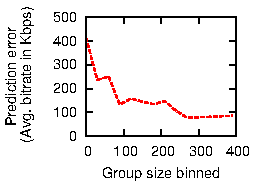
\includegraphics[width=110pt]{figures/count-err.pdf}
	\label{subfig:group-size-impact:count-err}
}
\subfigure[Distribution of group size]
{
        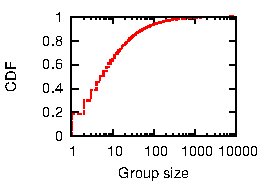
\includegraphics[width=110pt]{figures/count-cdf.pdf}
}
\tightcaption{Impact of group size (i.e., number of samples in a group). They show that more samples give more accuracy, but most of groups do not have sufficient samples for accurate prediction.}
\label{fig:group-size-impact}
\end{figure}

\item \emph{Bias} due to missing or unused information: The bias occurs when we do not observe (or use) an attribute that is important for prediction. Bias is not alleviated by gathering data from more session, but by gathering more attributes from each session.

\item \emph{Unavailability of recent data:} In a practical system, there are delays in measuring, sending and processing quality samples, so they are not available instantly.  If conditions change rapidly, there may be no quality samples sufficiently close to the session under prediction.  This is an extreme example of estimation error.  In this case it may be necessary to model the evolution of the video ecosystem over time in order to extrapolate to the current time. Figure~\ref{fig:quality-variability} shows per-minute quality variability. It shows that even with sufficient data, the mean value of a group of quality samples could vary significantly. This clearly indicates that any practical algorithm has to be running in real-time (on the order of one minute or less).

\begin{figure}[h!]
\centering
 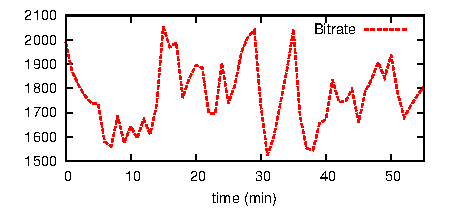
\includegraphics[width=0.4\textwidth] {figures/quality-time.pdf}
\tightcaption{Temporal variability of quality. The figure shows the mean value of average bitrate of a fixed group of same [Site, Initial CDN, Initial Bitrate, ConnectionType, ASN, Object], which has 100 quality samples in every minute in the figure.}
\label{fig:quality-variability}
\end{figure}

  \item \emph{Noise:} Even if we observed all conceivable attributes of a session and had infinitely many examples of exactly quality samples, outcomes may be affected by non-deterministic inputs.  For example, performance may be affected by exponentially backoff at the data link layer or the congestion generated by cross traffic at the network layer. This implies that some degree of prediction error is inevitable.
\xil{can i say this is Bias? because we do not capture this feature, and it is hard for us to extract a feature out of it, we consider it as noise?}
\end{packedenumerate}

Thus for any practical algorithm, it is a challenge to manage prediction error, which we will elaborate in the following section.

\tightsubsection{AC Aggregation and Challenges}
\label{subsec:aggregation}
A simple strategy to reduce estimation error is {\it aggregation}.  By aggregation we mean putting quality samples into coarser groups that match on only a subset of observed attributes.  Aggregation increases the number of samples in each identical group by reducing the number of attributes, thus reducing estimation error at the cost of increased bias. 
Intuitively, when estimation error is small (say, when a fine-grained identical group contains many sessions) we want to eliminate bias by using a fine-grained group.  When estimation error is large, we want to aggregate more. 
Then the question becomes how to determine the best level of aggregation.


\begin{figure}[h!]
\centering
 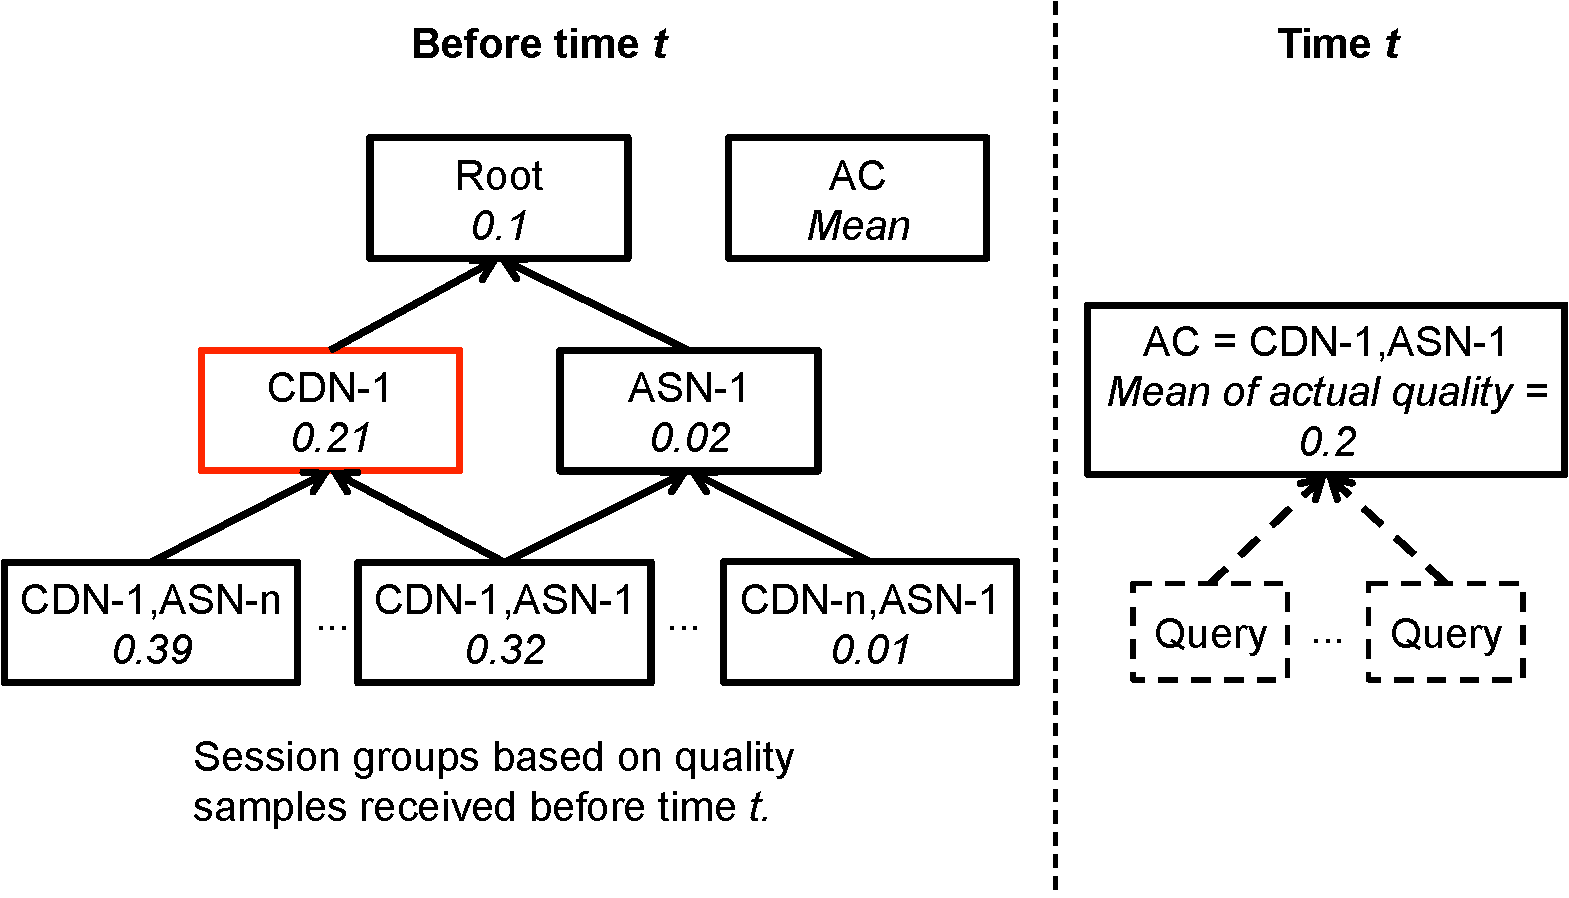
\includegraphics[width=0.5\textwidth] {figures/fig-optimal-AC.pdf}
\tightcaption{Example of how optimal AC is identified. The optimal AC is colored in red. The optimal AC for an identical group of sessions under prediction is the one of which the mean minimizes the prediction error.}
\label{fig:example-optimal-ac}
\end{figure}

\myparatight{Optimal AC} We use a simple oracle methodology, called {\it optimal AC}, to show the dynamics of the best level of aggregation. We assume an prediction algorithm with a delay of one minute, i.e., it predicts with information (quality samples) collected from previous minute.

Figure~\ref{fig:example-optimal-ac} shows an example of optimal AC with three attributes. For a finest identical group (e.g., $[CDN1,ASN1,Site1]$) at $t$-th minute, we first build a hierarchy that consists of all degrees of aggregation over the quality samples we collects before the $t$-th minute (e.g., the left part of Figure~\ref{fig:example-optimal-ac}). 
Remember that the optimal prediction of this identical group is its mean (see \Section~\ref{subsec:lowerbound}). 
Then, the optimal AC for this identical group is the degree of aggregation that gives the prediction value closest to the optimal prediction for the finest identical group at $t$-th minute. 
For instance, in Figure~\ref{fig:example-optimal-ac}, if the optimal prediction of the targeted identical group is 0.2, the optimal AC (colored in red) is the one with the closest prediction to 0.2, i.e., $(ASN, CDN)$. 

Note that optimal AC is not a real algorithm but an oracle analysis because the result depends on the underlying best prediction of sessions under prediction. It reflects the degree of aggregation of historical data that gives the best prediction for future (i.e., next minute's) sessions.
To show the dynamics of optimal AC, we present some empirical analysis results over our dataset from three aspects. 

\begin{figure}[h!]
\centering
\subfigure[Distribution of coverage of top five optimal ACs (w.r.t averge bitrate).]
{
        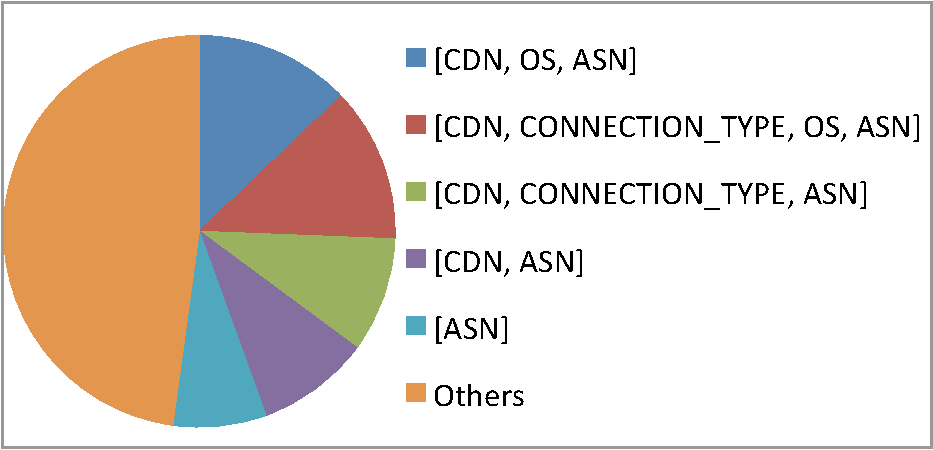
\includegraphics[width=0.4\textwidth]{figures/optimal_AC_distribution.pdf}
}
\subfigure[Optimal AC prevalence.]
{
        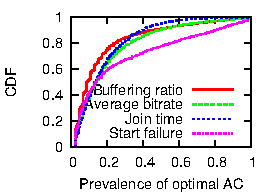
\includegraphics[width=0.24\textwidth]{figures/optimal-prevalence.pdf}
}
\hspace{-0.6cm}
\subfigure[Optimal AC persistence.]
{
        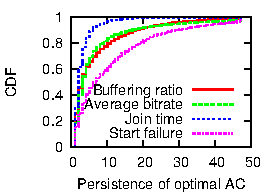
\includegraphics[width=0.24\textwidth]{figures/optimal-persistence.pdf}
}
\tightcaption{Dynamics of the optimal AC. (a) gives coverage of optimal ACs (for each AC, the fraction of sessions of which this AC is the optimal AC).
(b) gives prevalence of pair of (session under prediction, optimal AC) (the fraction of time that the finest group has this optimal AC).
(c) gives persistence of pair of (session under prediction, optimal AC) (i.e., the longest continuous duration where a finest group has the same optimal AC).}
\label{fig:optimal-ac-dynamics}
\end{figure}


 
\begin{packeditemize}
	\item {\it No single optimal AC:} Figure~\ref{fig:optimal-ac-dynamics}-(a) shows the coverage of optimal ACs, i.e., the fraction of time for which a given AC is the optimal AC. Note that there is no single optimal AC. For example, the finest group only has coverage about 20\% and no coarsest grain AC (single attribute) is among the top 5. This implies that the optimal AC is often in between.
	\item {\it No temporally prevalent optimal AC:} Figure~\ref{fig:optimal-ac-dynamics}-(b) shows the prevalence of the $($\emph{session-under-prediction, optimal AC}$)$ pairs, i.e., the fraction of time the fines group of sessions has the same optimal AC. Note that $70\%$ pairs only last for less than $20\%$ of time. This implies that there is no single or a small set of optimal ACs that can cover most sessions.
	\item {\it Highly dynamic optimal ACs:} Figure~\ref{fig:optimal-ac-dynamics}-(c) shows the persistence of the $($\emph{session-under-prediction, optimal AC}$)$ pairs, i.e., the longest continuous duration where the finest group has the same optimal AC. Only 40\% of pairs last for more than 10 minutes. This suggests that even with a reactive strategy will be challenging to track the optimal ACs.
\end{packeditemize}

To conclude, we find that the optimal AC (the aggregation that gives minimal prediction error) is in many cases neither the finest nor the coarsest one, and, in addition, is highly dynamic. This presents a challenge in designing a practical prediction algorithm to identify the best AC in real-time.


